\documentclass{beamer}
\usepackage[utf8]{inputenc}
\usepackage{xcolor}
\usepackage[T1]{fontenc}
\usepackage[normalem]{ulem}
\usetheme{Antibes}

\title{Projet Optimisation :\\Support Vector Machine}
\author{K. Kamtue \& Cl. Réda}
\institute{\textsc{ENS Cachan}}
\date{\today}

\setbeamerfont{page number in head/foot}{size=\large}
\setbeamertemplate{footline}[frame number]

\begin{document}
\maketitle
\tableofcontents
\setlength{\parindent}{1cm}

\section{Description du projet}

\subsection{Sujet}

\begin{frame}
\tableofcontents[currentsubsection]
\end{frame}

\begin{frame}
\frametitle{Sujet}
\framesubtitle{\emph{Support Machine Vector}}

\begin{alertblock}{Objectif}
\begin{center}
Faire de l'apprentissage supervisé
\end{center}
\end{alertblock}

\pause

\begin{itemize}
\item Appliqué à la \textbf{classification binaire} ($y_i \in \{1, -1\}$);

\pause

\item Recherche d'une \textbf{frontière linéaire} $f : x \rightarrow \omega^Tx$ vérifiant :

         \begin{center}
         $\forall i, y_i = -1 \Rightarrow f(x_i) < 0$\\
         $\forall i, y_i = 1 \Rightarrow f(x_i) > 0$\\
         $\Leftrightarrow \forall i, y_i \times f(x_i) > 0$ (1)
         \end{center}
\end{itemize}

\end{frame}

\begin{frame}
\frametitle{Sujet}
\framesubtitle{\emph{Support Machine Vector}}

         \begin{figure}
         \centering
         \caption{Exemple avec deux classes (rouge et bleue)}
         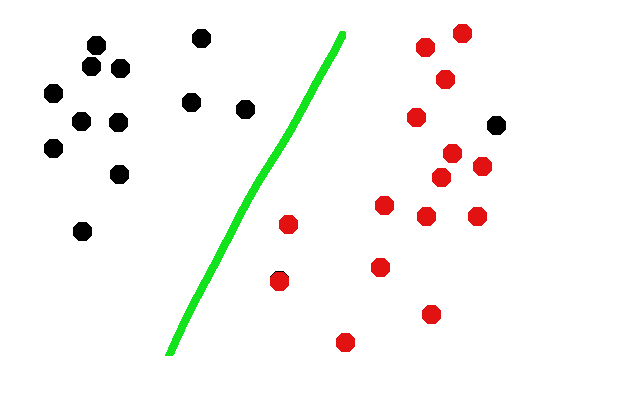
\includegraphics[scale=0.4]{images/voronoi.png}
         \end{figure}

\end{frame}

\subsection{Le problème d'optimisation}

\begin{frame}
\frametitle{Le problème d'optimisation}
\framesubtitle{Recherche du problème d'optimisation}

\begin{block}{Le problème d'optimisation (naïvement)}
$\gamma$ : distance entre les droites $f(x) = 1$ et $f(x) = -1$ (\textbf{marge}).

\pause

      \begin{center}
        $max_{w}$ $\gamma = \frac{2}{\|w\|}$\\
        avec $\forall i, y_i \times f(x_i) > 0$\\

\pause

       \bigskip
        $\Leftrightarrow min_{w}$ $\frac{1}{2} \|w\|^2$\\
        avec $\forall i, y_i \times f(x_i) > 0$\\
      \end{center}

\end{block}

\textbf{Attention :} si l'ensemble n'est pas \underline{séparable} !

\end{frame}

\begin{frame}
\frametitle{Le problème d'optimisation}
\framesubtitle{Recherche du problème d'optimisation}

         \begin{figure}
         \centering
         \caption{Exemple avec deux classes (rouge et bleue)}
         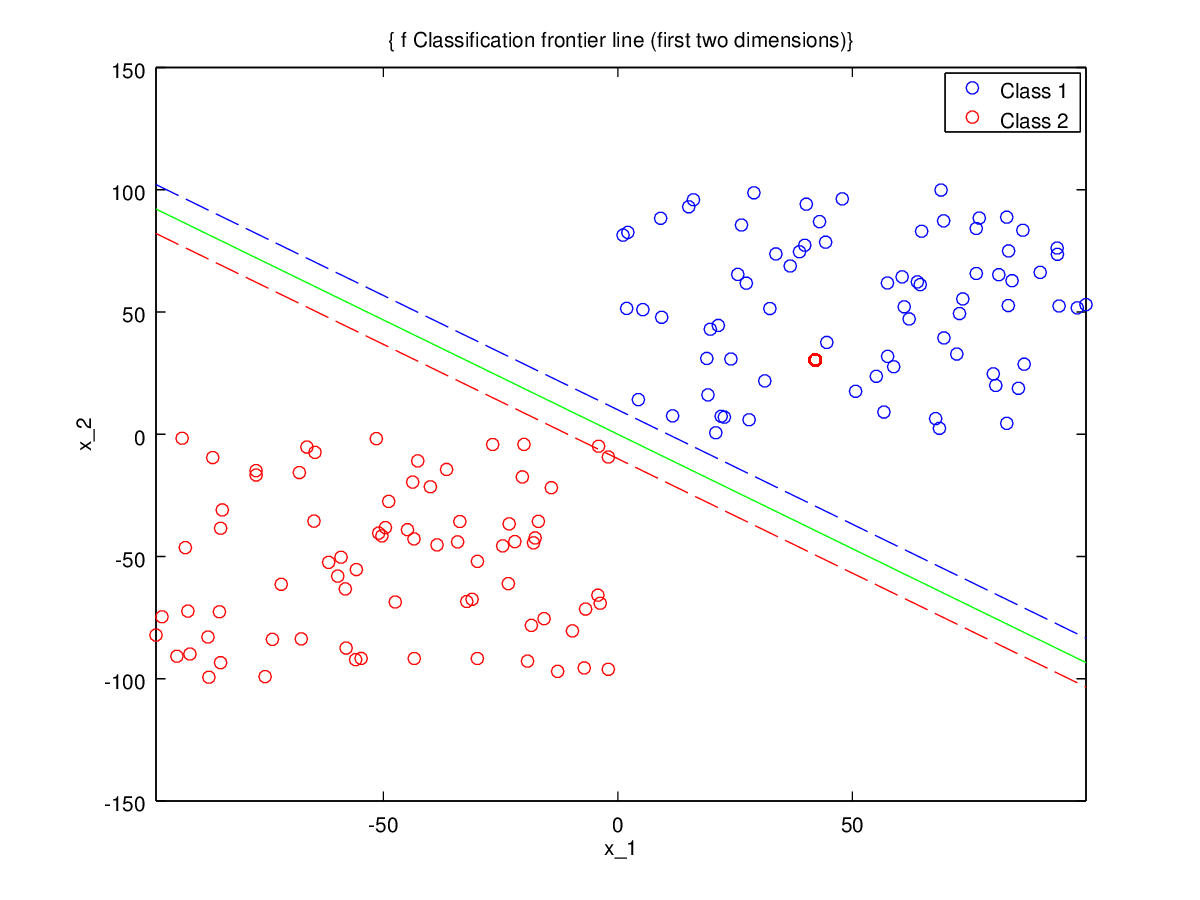
\includegraphics[scale=0.4]{images/voronoi2.png}
         \end{figure}

\end{frame}

\begin{frame}
\frametitle{Le problème d'optimisation}
\framesubtitle{Adaptation au cas non séparable}

Soit $z_i = max(0, 1-y_i \times f(x_i))$ (perte de \textbf{Hinge}).

\pause

\bigskip

\begin{block}{En rendant le problème toujours faisable et convexe}

Pénaliser les erreurs de classification avec les $(z_i)_i$ et $C$ :

           \begin{center}
           $min_{w, z}$ $\frac{1}{2} \|w\|^2 + C \sum_{i \leq m}z_i$\\
           avec $\forall i, z_i \geq 0$\\
           $\forall i, y_i \times (\omega^{T} x_i) \geq 1 - z_i$\\
           \end{center}

\end{block}

\end{frame}

\subsection{Implémentation}

\begin{frame}
\tableofcontents[currentsubsection]
\end{frame}

\begin{frame}
\frametitle{Implémentation}
\framesubtitle{Résolution du problème d'optimisation}

\begin{itemize}
\item Utilisation de la \textbf{méthode de Newton} pour trouver $\omega$ :

\bigskip

\begin{block}{Rappel : Mise à jour du vecteur $x$ cherché avec la \textbf{méthode de Newton}}
          \begin{center}
          $x_{n+1} \leftarrow x_{n} + s \times \nabla^2 obj(x_n)^{-1}\nabla obj(x_n)$
          \end{center}

  (ici, en cherchant $s$, taille du pas, par \textbf{backtracking line search})
\end{block}

\pause

\item Utiliser la \textbf{méthode de la barrière logarithmique}.
% pour pouvoir utiliser la méthode de Newton sur un problème non contraint

\pause

\item Rendre le problème indépendant de la \textbf{dimension};
%(\textbf{dépendant du nombre d'échantillons} !) en résolvant le \emph{problème dual}; pour une meilleure complexité temporelle

\end{itemize}

\end{frame}

\begin{frame}
\frametitle{Implémentation}
\framesubtitle{Indépendance en la dimension des points : \textbf{problème dual}}

Après calcul du lagrangien et minimisation en $\omega$ : 
%($\lambda$ multiplicateur de Lagrange) :

\pause

\begin{block}{\textbf{Problème dual}}
             \begin{center}
             $max_{\lambda \in \mathbb{R}^{+m}} -\frac{1}{2}\|\sum_i\lambda_iy_ix_i\|^2_2 + $\textbf{1}$^T\lambda$\\ 
             avec $\forall i, 0 \leq \lambda_i \leq C$\\
             (par les conditions de KKT)
             \end{center}
\end{block}

\pause

\begin{alertblock}{Obtenir la solution du primal à partir de celle du dual}
             \begin{center}
               $\omega^{*} = \sum_i \lambda^{*}_i y_i x_i$
             \end{center}
\end{alertblock}

\end{frame}

\begin{frame}
\frametitle{Implémentation}
\framesubtitle{Rendre le problème indépendant de la dimension}

Utilisation de l'\emph{astuce du noyau} :

\bigskip

\begin{block}{Problème dual}
Soit $K = X^TX$ (noyau linéaire). Alors :

\bigskip
                 \begin{center}
                 $max$ $-\frac{1}{2}\lambda^Tdiag(y)Kdiag(y)\lambda+$\textbf{1}$^T\lambda$\\
                 avec $\forall i, 0 \leq \lambda_i \leq C$ 
                 \end{center}
\end{block}

\end{frame}

\begin{frame}
\frametitle{Implémentation}
\framesubtitle{Supprimer les contraintes d'inégalité}

Utilisation de la \textbf{méthode de la barrière logarithmique} :

\pause

\begin{block}{Fonction barrière pour éliminer les contraintes d'inégalité}
          \begin{center}
          $\Phi(\lambda) = \sum_i (- log(C - \lambda_i) - log(\lambda_i))$\\
          $= - \sum_i log((C - \lambda_i)\lambda_i)$ 
          \end{center}
\end{block}

\pause

\begin{alertblock}{Problème d'optimisation final}
          \begin{center}
          $max$ $-\frac{1}{2}\lambda^Tdiag(y)Kdiag(y)\lambda+$\textbf{1}$^T\lambda + \Phi(\lambda)$\\ 
          \end{center}
\end{alertblock}

\end{frame}

\section{Résultats}

\subsection{Détails de l'implémentation}

\begin{frame}
\tableofcontents[currentsubsection]
\end{frame}

\begin{frame}
\frametitle{Détails de l'implémentation}
\framesubtitle{Tracé de la convergence de la méthode de Newton}

% CV linéaire au début, puis quadratique, comme vu en cours

         \begin{figure}
         \centering
         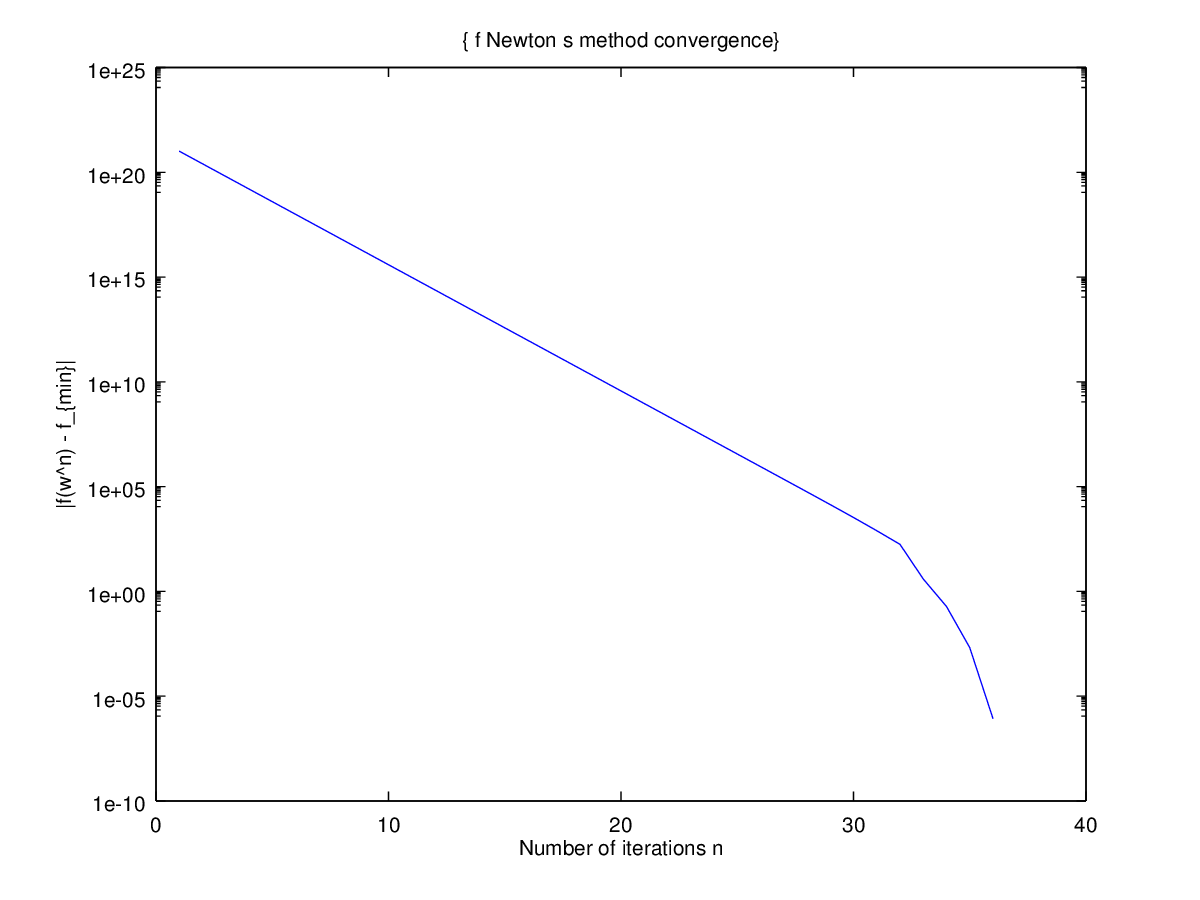
\includegraphics[scale=0.4]{images/cvnewton4.png}
         \end{figure}

\end{frame}

\begin{frame}
\frametitle{Détails de l'implémentation}
\framesubtitle{Dépendance en la taille de l'échantillon}

% On voit que la convergence est très lente quand la taille est grande
% Par contre, il y a indépendance de la dimension des échantillons 

         \begin{figure}
         \centering
         \caption{Comparaison des temps de calcul selon $n$ et $d$\\
                 Ensemble | C | $d$ | $n$ | Nb d'itérations | temps}
         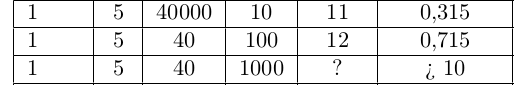
\includegraphics[scale=0.6]{images/tabl2.png}
         \end{figure}

\end{frame}

\begin{frame}
\frametitle{Détails de l'implémentation}
\framesubtitle{Accélération de la convergence quand $C$ augmente}

% POURQUOI ?!

         \begin{figure}
         \centering
         \caption{Evolution du temps de calcul en fonction de C}
         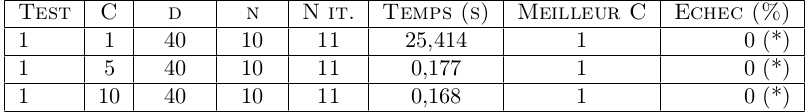
\includegraphics[scale=0.4]{images/tabl1.png}
         \end{figure}

\end{frame}

\subsection{Tracé de la frontière de classification}

\begin{frame}
\tableofcontents[currentsubsection]
\end{frame}

\begin{frame}
\frametitle{Tracé de la frontière de classification}
\framesubtitle{Pour $C = 5, n = 150, d = 200$}

Points centrés réduits avec des fonctions gaussiennes (2D) :

         \begin{figure}
         \centering
         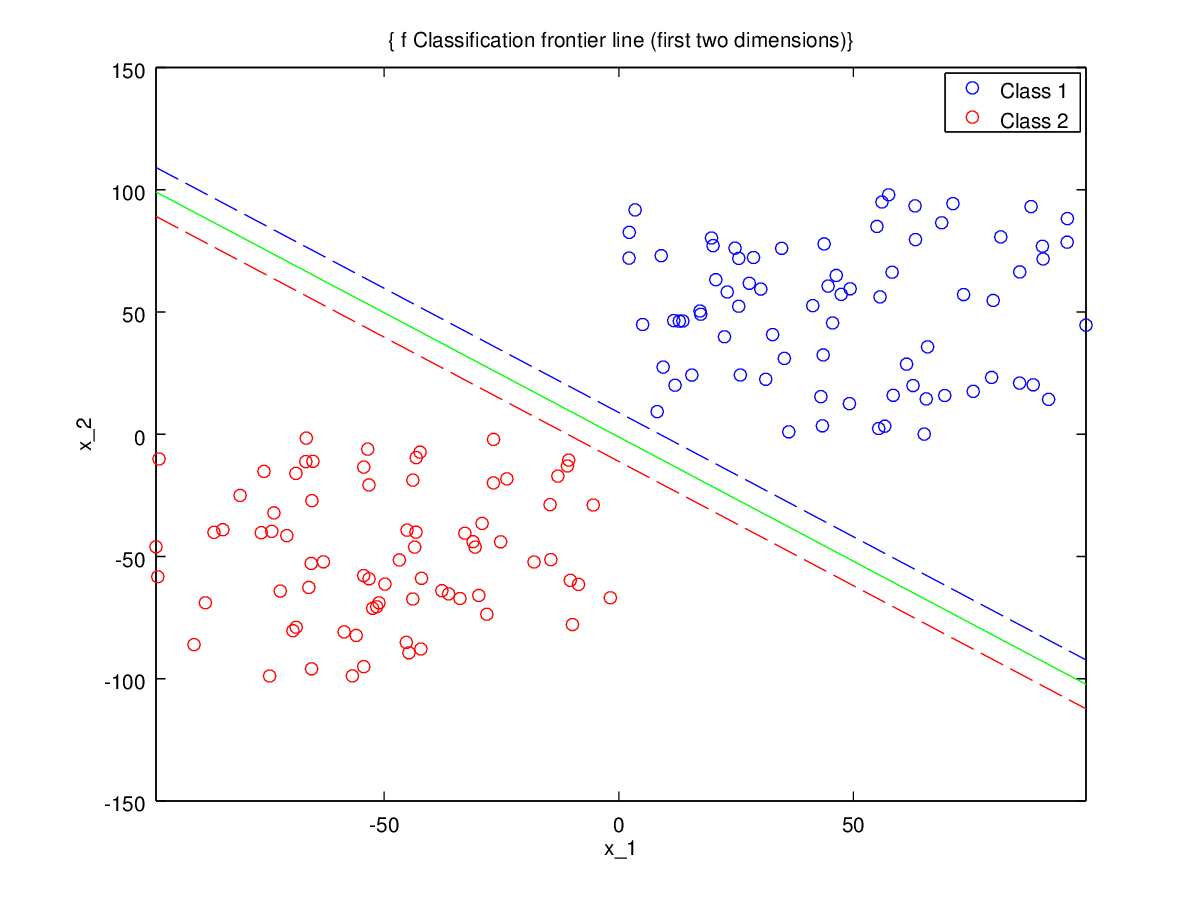
\includegraphics[scale=0.4]{images/line4.png}
         \end{figure}

\end{frame}

\begin{frame}
\frametitle{Tracé de la frontière de classification}
\framesubtitle{Pour $C = 5, n = 150, d = 200$}

Points centrés réduits avec des fonctions gaussiennes (3D) :

         \begin{figure}
         \centering
         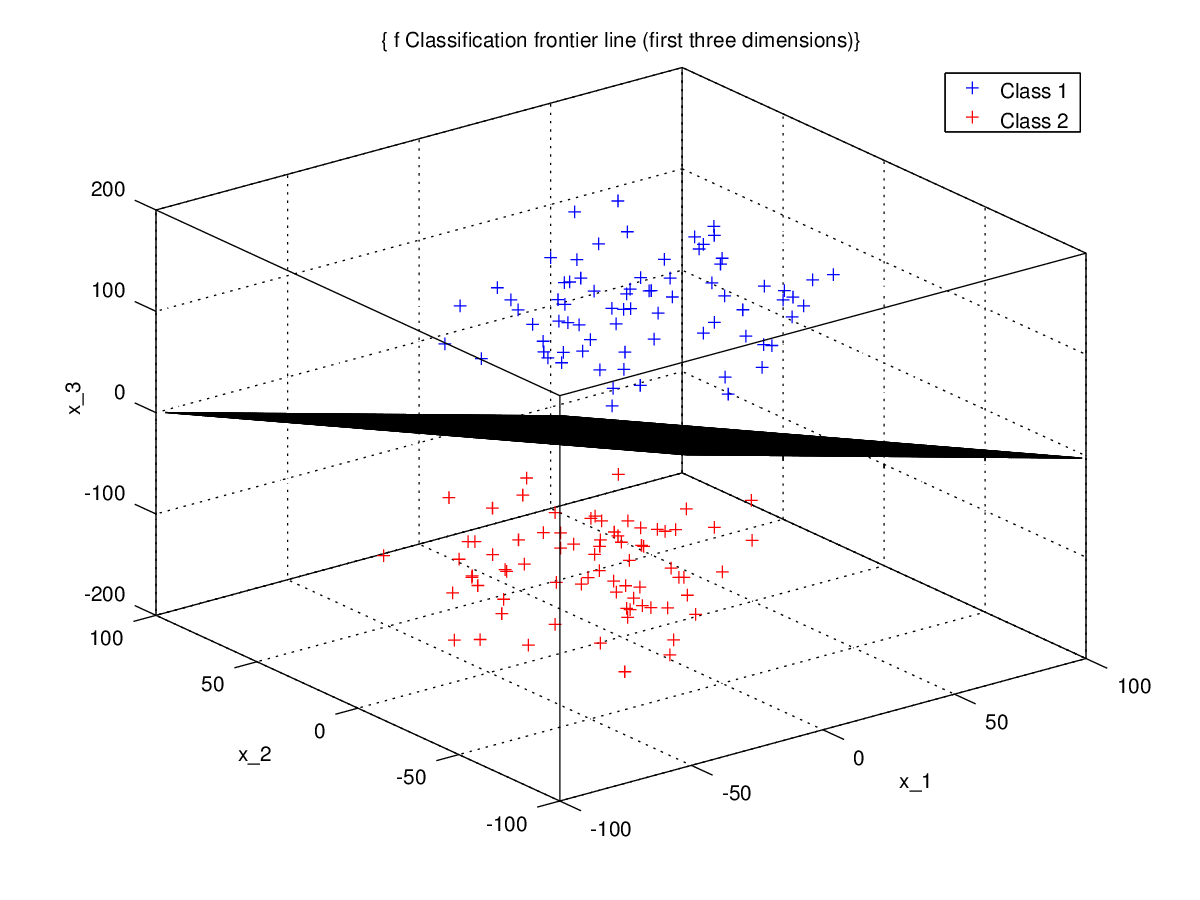
\includegraphics[scale=0.4]{images/plane4.png}
         \end{figure}

\end{frame}

\begin{frame}
\frametitle{Tracé de la frontière de classification}
\framesubtitle{Pour $C = 5, n = 150, d = 200$}

Génération avec des fonctions gaussiennes (2D) :

         \begin{figure}
         \centering
         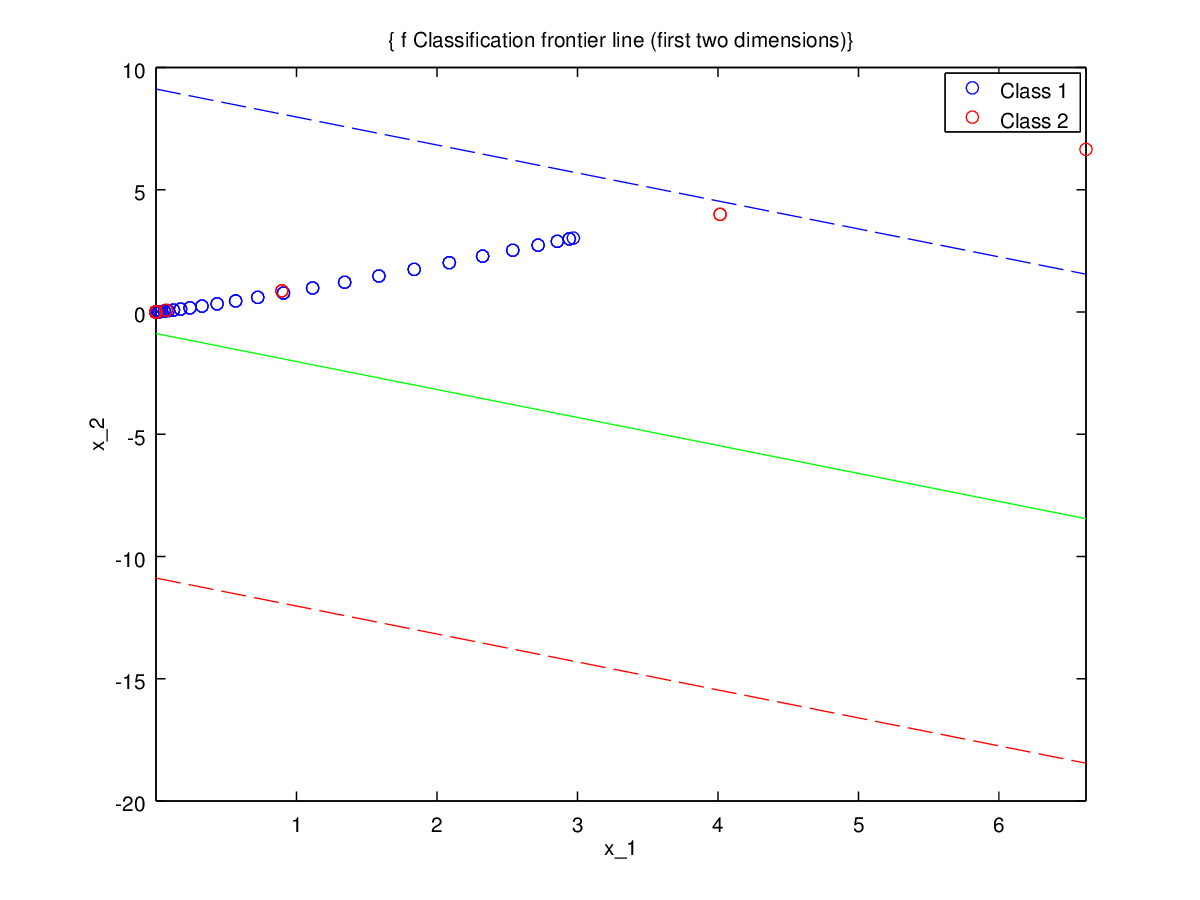
\includegraphics[scale=0.4]{images/line5.png}
         \end{figure}

\end{frame}

\begin{frame}
\frametitle{Tracé de la frontière de classification}
\framesubtitle{Pour $C = 5, n = 150, d = 200$}

Génération avec des fonctions gaussiennes (3D) :

         \begin{figure}
         \centering
         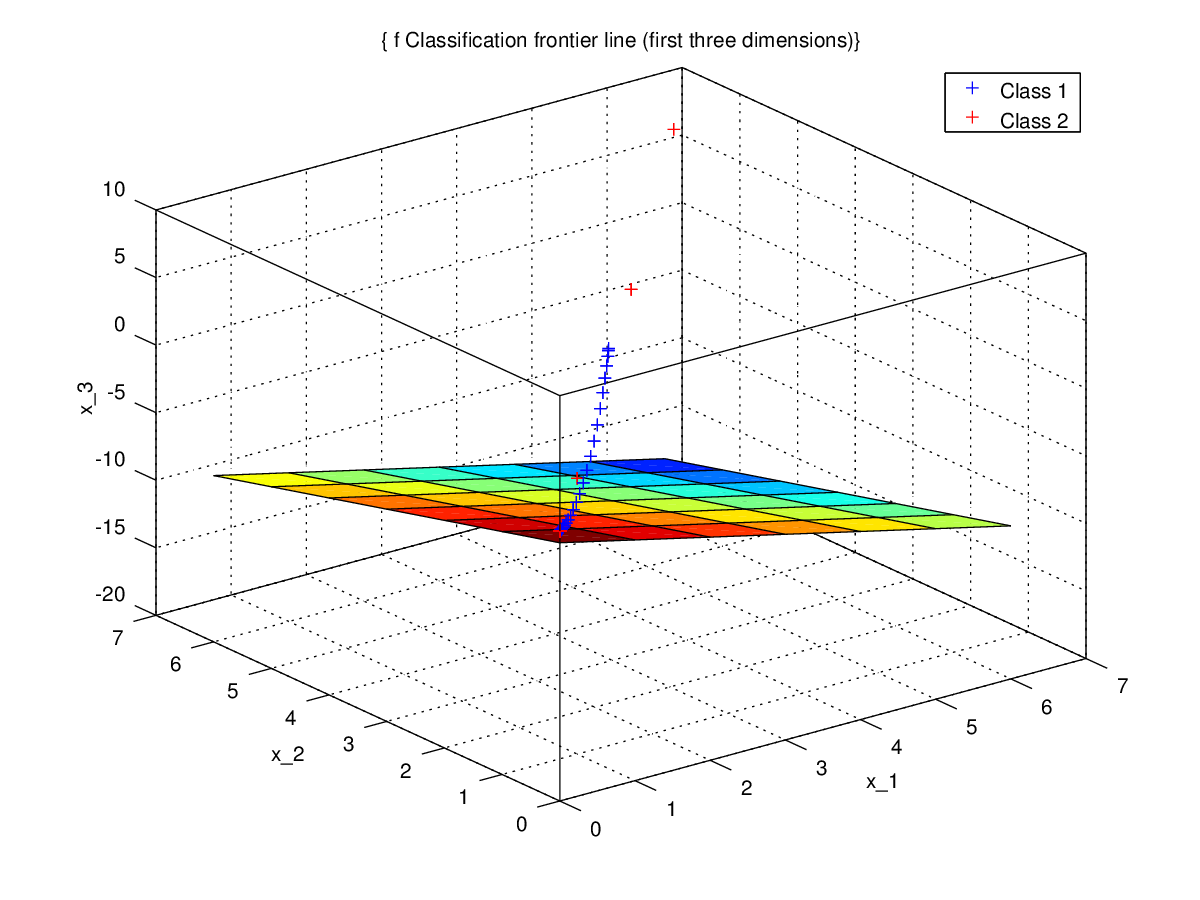
\includegraphics[scale=0.4]{images/plane5.png}
         \end{figure}

\end{frame}

\section{Extensions}

\begin{frame}
\tableofcontents[currentsection]
\end{frame}

\begin{frame}
\frametitle{Extensions}
\framesubtitle{Ajouts au projet}

\begin{itemize}
\item \textbf{Validation croisée} (choix de la meilleure valeur de C);

% Prend beaucoup de temps, technique de leave-one-out

\pause

\item Implémentation de \textbf{Coordinate Descent};

% Plus rapide que l'algorithme original POURQUOI ?!

\pause

\item Implémentation de \textbf{ACCPM};

% Des erreurs de précision et un problème au niveau de l'implémentation
% du constraint dropping
\end{itemize}

\end{frame}

\section{Démonstration}

\begin{frame}
\tableofcontents[currentsection]
\end{frame}

\begin{frame}

\bigskip

\bigskip

\begin{center}
\textbf{Démontration du SVM}
\end{center}

\end{frame}

% Générer selon les trois méthodes et tracer la frontière de classification

% Préparer les sets de test à l'avance

\end{frame}


\end{document}
